% MA211 - Lecture 07
\documentclass[pdftex, xcolor=pdftex, dvipsnames, handout]{beamer}

\usetheme{MA211}
\usepackage{thumbpdf}
\usepackage{wasysym}
%\usepackage{ucs}
\usepackage[utf8]{inputenc}
\usepackage{pgf,pgfarrows,pgfnodes,pgfautomata,pgfheaps,pgfshade}
\usepackage{verbatim}

\usepackage{eurosym}
\usepackage{euler}

\usepackage{calc}               % Simple computations with LaTeX variables
%\usepackage[hang]{caption2}     % Improved captions

\usepackage{graphicx}           % Standard graphics package

\usepackage{amsmath, amsthm, amssymb}


\newcommand{\fquad}{\mbox{\qquad}}
\newcommand{\bull}{$\bullet$ }

\newcommand {\I} {\mathcal I}
\newcommand {\calI} {\mathcal I}
\def\disint{\displaystyle\int}

\DeclareMathOperator{\D}{d}
\newcommand{\dydx}{\frac{\D y}{\D x}}

%\definecolor{gray}{rgb}{0.69, 0.69, 0.69} \newcommand{\gray}[1]{\textcolor{gray}{#1}}
\definecolor{dogreen}{rgb}{0.33, 0.42, 0.18} \newcommand{\dogreen}[1]{\textcolor{dogreen}{#1}}
\definecolor{maroon}{rgb}{.5,0.2,0.2}\newcommand{\maroon}[1]{\textcolor{maroon}{#1}}
\definecolor{greena}{rgb}{.1,0.581,0.1}\newcommand{\greena}[1]{\textcolor{greena}{#1}}

\definecolor{blue4}{rgb}{0,0,.545}
\newcommand{\Blue}[1]{\textcolor{blue}{#1}}
\newcommand{\Red}[1]{\textcolor{red}{#1}}
\definecolor{pink}{rgb}{1.,0.75,0.8}
\definecolor{darkred}{rgb}{0.5,0.0,0.0}
\definecolor{darkgreen}{rgb}{0,0.3,0.3}
\definecolor{purple}{rgb}{0,0.3,0.3}
\definecolor{darkblue}{rgb}{0.0, 0.0, .5}
\definecolor{dpurple}{rgb}{.3,.0,.3}
\newcommand{\Green}[1]{\textcolor{darkgreen}{#1}}
\newcommand{\DRed}[1]{\textcolor{darkred}{#1}}
\newcommand{\DBlue}[1]{\textcolor{darkblue}{#1}}
\newcommand{\Purple}[1]{\textcolor{dpurple}{#1}}
\newcommand{\Emph}[1]{\textcolor{darkred}{\textbf{\it #1}}}
\newcommand{\remph}[1]{\textcolor{darkred}{\textbf{\emph{#1}}}}
\newcommand{\bemph}[1]{\textcolor{darkblue}{\textbf{\emph{#1}}}}
\newcommand{\gemph}[1]{\textcolor{darkgreen}{\textbf{\emph{#1}}}}
\newcommand{\Bf}[1]{\textcolor{darkblue}{\textbf{#1}}}
\newcommand{\Gf}[1]{\textcolor{darkgreen}{\textbf{#1}}}
\newcommand{\Rf}[1]{\textcolor{red}{\textbf{#1}}}
\newcommand{\Rmf}[1]{\textcolor{red}{\mathbf{#1}}}

\newcommand{\Conj}[1]{\overline{#1}}

\newcommand{\code}[1]{\textcolor{darkblue}{\texttt{\textbf{#1}}}}
\newcommand{\icode}[1]{{\blue\texttt{\textbf{\emph{#1}}}}}
\newcommand{\gcode}[1]{{\Green{\texttt{\textbf{\emph{#1}}}}}}
\newcommand{\out}[1]{\texttt{\emph{\textbf{\Green{#1}}}}}





\newenvironment{vminipage}%
{\begin{Sbox}\begin{minipage}\begin{small}\begin{verbatim}}%
{\end{verbatim}\end{small}\end{minipage}\end{Sbox}\fbox{\TheSbox}}

\newenvironment{nminipage}%
{\begin{Sbox}\begin{minipage}}%
{\end{minipage}\end{Sbox}\fbox{\TheSbox}}


\let\Arg\relax\DeclareMathOperator{\Arg}{\mathtt{Arg}}
\let\Arg\relax\DeclareMathOperator{\e}{\mathtt{e}}

\newcommand {\AND} {\wedge}
\newcommand {\OR} {\vee}
\newcommand {\NOT} {\neg}
\newcommand {\IMPLIES} {\rightarrow}
%\newcommand {\IFF} {\leftrightarrow}
\renewcommand {\iff} {\Leftrightarrow}
\newcommand {\NAND} {\uparrow}
\newcommand {\NOR} {\downarrow}
\newcommand {\XOR} {\otimes}

\newenvironment{citemize}% Colour items
{\begin{description}}%
{\end{description}}

\newcommand {\maroonitem}{\item[\maroon{$\bullet$}]}

\newcommand {\gitem} {\item {\includegraphics[width=.4cm,angle=-10]{img/green-bullet-on-white.ps}}}
\newcommand {\ritem} {\item {\includegraphics[width=.4cm,angle=-10]{img/red-bullet-on-white.ps}}}
\newcommand {\yitem} {\item {\includegraphics[width=.4cm,angle=-10]{img/yellow-bullet-on-white.ps}}}
\newcommand {\bitem} {\item {\includegraphics[width=.4cm,angle=-10]{img/blue-bullet-on-white.ps}}}

\newcommand {\greenitem} {\item {\includegraphics[width=.4cm,angle=-10]{img/green-bullet-on-white.ps}}}
\newcommand {\reditem} {\item {\includegraphics[width=.4cm,angle=-10]{img/red-bullet-on-white.ps}}}
\newcommand {\yellowitem} {\item {\includegraphics[width=.4cm,angle=-10]{img/yellow-bullet-on-white.ps}}}
\newcommand {\blueitem} {\item {\includegraphics[width=.4cm,angle=-10]{img/blue-bullet-on-white.ps}}}

\newcommand {\eq}[1]%
  {$\DBlue{#1}$}
\newcommand {\eqd}[1]%
  {$\displaystyle\DBlue{#1}$}
%\newcommand{\eq}[1]{\boldmath \DBlue{$#1$}}


\newcommand {\csf}{\centerslidesfalse}
\newcommand {\cst}{\centerslidestrue}

\newcommand {\vecii}[2] {   \big(\begin{smallmatrix} #1 \\ #2 \end{smallmatrix}\big)}
\newcommand{\atwo}[2]{\left(\!\!\begin{array}{c} #1 \\ #2 \end{array}\!\!\right)}


\newcommand{\C}{\mathbb{C}}
\newcommand{\Q}{\mathbb{Q}}
\newcommand{\R}{\mathbb{R}}
\newcommand{\N}{\mathbb{N}}
\newcommand{\Z}{\protect\mathbb{Z}}  % protect for index.
\newcommand {\Rs}{ \mathbb{R}}
\newcommand {\Cs}{ \mathbb{C}}
\newcommand {\Rnn}{ \mathbb{R}^{n \times n}}
\newcommand {\Rn}{ \mathbb{R}^{n}}


\newcommand{\mblock}{%
\setbeamercolor*{block title}{bg=maroon,fg=white}
\setbeamercolor*{block body}{bg=white,fg=maroon}
}%

\newcommand{\bblock}{%
\setbeamercolor*{block title}{bg=Steel,fg=white}
\setbeamercolor*{block body}{bg=Mylightgray,fg=Steel}
}%

\newcommand{\gblock}{%
\setbeamercolor*{block title}{bg=Green,fg=white}
\setbeamercolor*{block body}{bg=Mylightgray,fg=darkgreen}
}%


\newcommand{\rblock}{%
\setbeamercolor*{block title}{bg=Red,fg=white}
\setbeamercolor*{block body}{bg=white,fg=Black}
}%


\newcommand{\TakeNotes}{
\includegraphics[width=2cm]{TakeNote}}

\def\eps{\varepsilon}
\newcommand {\del}[2]{ {\frac{\partial #1}{\partial #2}}}
\newcommand {\x}[1]{x^{[#1]}}
\newcommand {\delx}{ {\frac{\partial}{\partial x}}}
\newcommand {\delt}{ {\frac{\partial}{\partial t}}}
\newcommand {\dely}{ {\frac{\partial}{\partial y}}}
\newcommand {\ith}{{(i)}}
\renewcommand {\vec}[1]{ {\boldsymbol{#1}}}
\newcommand {\Oh} {\mathcal O}
\newcommand {\Err} {\mathcal E}
%\newcommand {\th} {\mathrm{th}}
\DeclareMathOperator{\fl}{fl}
\DeclareMathOperator{\sign}{sign}
\DeclareMathOperator{\Cond}{Cond} 
\DeclareMathOperator{\cond}{cond}
\DeclareMathOperator{\diag}{diag} 
\DeclareMathOperator{\sym}{sym} 
\DeclareMathOperator{\Trace}{Trace}
\DeclareMathOperator{\E}{e}

\newcommand {\Rsym}{{ \mathbb{R}^{n \times n}_\mathrm{sym}}}

\newcommand {\st} {\mathrm{st}}
\newcommand {\nd} {\mathrm{nd}}


\parskip .25cm


\theoremstyle{definition}
\newtheorem{exercise}{Exercise}[section]
\newtheorem{method}{Method}[section]

\newcommand{\Header}[1]{\begin{center}{\Large \Bf{#1}}\end{center}}

\subtitle{MA211}
\title{Lecture 7: Logs and Exponentials}

\author{Dr Niall Madden}

\date{\Large Mon 29 September 2008}


\begin{document}


\frame{

\begin{block}{}
\begin{center}
{\large \insertsubtitle}

\vspace{.1cm}

\begin{Large}
\textbf{\inserttitle}
\end{Large}

\vspace{.15cm}

% {\footnotesize \insertauthor}

\vspace{.3cm}

{ {\insertdate}}
\end{center}
\end{block}


\vspace{-0.25cm}
\begin{center}
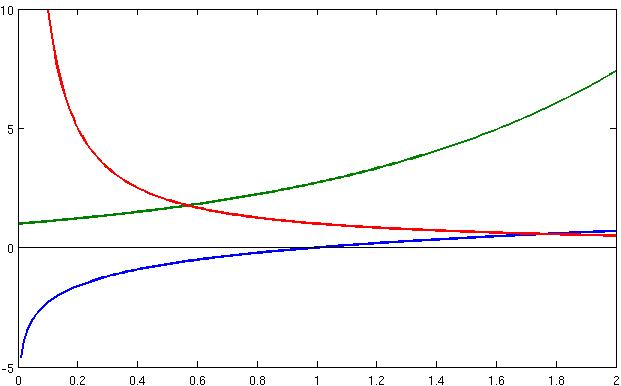
\includegraphics[height=4cm]{images/log}

\end{center}
}


\frame{

\Header{Reminder: Problem Set 1}

Problem Set 1 is now available from the web-site.

Write out,  clearly  and carefully, solutions to the selected
exercises and submit them at our lecture on Monday, Oct 6th.


\pause
Tutorials take place
\begin{itemize}
\item Tuesday, 3pm, AC202

\item Wednesday, 5pm, QA003 (Physiology lecture room)
\end{itemize}


}

\frame{
  \frametitle{In today's lecture}
 \tableofcontents

}





\section{Order of a Differential Equation}

\frame{

There are different types of differential equation that we will study
in this course. 

The first way of classifying a DE is according to the number of
derivatives present.

\begin{definition}[Order]
The \Bf{Order} of a differential equation is the order of the highest
derivative present.
\end{definition}

\pause
\Emph{Examples:}

\vspace{1cm}

\pause
In this course we'll only consider \eqd{1^\st}- and \eqd{2^\nd}-order DEs.


}

\section{Initial and Boundary Value Problems}

\frame{

There is a further way of classifying DEs to which we seek a 
\Emph{particular solutions}.


\begin{enumerate}
\item Initial Value Problems

\item Boundary Value Problems

\end{enumerate}

}


\subsection{IVPs}

\frame{

\Bf{Examples:}


\vspace{4cm}

%\pause
Key idea:
\begin{definition}[IVP]
An \Bf{Initial Value Problem} is of the form:
\begin{quote}
Find a function \eq{f(t)} that satisfies a DE for all \eq{t \geq T}
and one or more of f(T), f'(T), f''(T)... are given.
\end{quote}

\end{definition}
}


\subsection{BVPs}

\frame{

\Bf{Examples:}


\vspace{4cm}

%\pause
Key idea:
\begin{definition}[BVP]
A \Bf{Boundary Value Problem} is of the form:
\begin{quote}
Find a function \eq{f(x)} that satisfies a DE for all \eq{x} in the
interval \eq{(a,b)} and f(a) and  f(b) are given.
\end{quote}

\end{definition}
}

\frame{
Mathematically, we will treat these as being the same:
\begin{enumerate}
\item Solve the differential Equation to get the \Emph{general solution},
  including constants of integration.

\item Use the initial or boundary values to solve for the constants
  and so get the \Emph{particular solution}.
\end{enumerate}

\Bf{Examples:}

\vspace{4cm}

}

\frame{

\begin{exercise}[7.1]
Find solutions to the following   differential equations
\begin{enumerate}[(i)]
\item $y'(t) = x-2$
\item  $f'(x) = x^{-2} - x^{-3}$ subject to $f(-1)=0$.
\item $y''(x) = x^3-1$, with \eq{y'(0)=0, y(0)=8}.
\item  $f''(t) + f(t) =0$. (Hint: Trig function)
\item $f''(t) = 9f(t)$  (Hint: Trig function)
\end{enumerate}
\end{exercise}
}

\section{Transcendental Functions}

\frame{
This course is mostly concerned with \Emph{functions}, and their
derivatives and integrals.

However, we've mostly just looked at polynomials and trigonometric functions
in any detail.

Most interesting functions that are solutions to differential
equations are \Emph{Transcendental}: they can't be made of addition
and multiplication of the independent variable.


The Trig functions are transcendental, as are the exponential and
logarithmic functions, and the hyperbolic functions.


First we'll cover \Bf{Inverse functions}.


%For more details: See \Bf{Chap 4} or Adams \emph{Calculus: a complete
%  course}.
}



\section{Inverse functions}

\frame{
Recall... 

\begin{definition}[One-to-one]
The function \eq{f:A \rightarrow B} is one-to-one  if
whenever \eq{f(a_1)= f(a_2)}  then \eq{a_1 =a_2}.
\end{definition}


% \begin{example}
% \begin{itemize}[<+->]

% \item The function \eq{f:\R \to \R} defined by \eq{f(x)=x^3} is
% \Bf{one-to-one}.

% \item The function \eq{f:\R \to \R} defined by \eq{f(x)=x^2} is
% \Emph{not} \Bf{one-to-one}.


% \item Let \eq{\R^+} denote the \alert{positive} real numbers.
% The function \eq{f:\R^+ \to \R^+} defined by \eq{f(x)=x^2} is
%  \Bf{one-to-one}.
% \end{itemize}
% \end{example}

%
%}
%
%\frame{

~


\begin{definition}[Onto]
The function \eq{f:A \rightarrow B} is onto if for each $y \in B$
there exists $x \in A$ such that $y$ is the image of $x$. 
\end{definition}

%\begin{example}
%The function \eq{f:\R \to \R} defined by \eq{f(x)=x^3} is
%\Bf{onto}.%
%
%The function \eq{f:\R \to \R} defined by \eq{f(x)=x^2} is
%\Emph{not} \Bf{onto}.
%
%The function \eq{f:\R^+ \to \R^+} defined by \eq{f(x)=x^2} is
% \Bf{onto}.
%%
%
%\end{example}

}


\frame{
When a function is both \alert{one-to-one} and \alert{onto} is has an
\Bf{Inverse}.

\begin{definition}
If the function \eq{g} is the \alert{inverse} of \eq{f} then 
\[
\text{ when } f(x)=y, \text{ we get that } g(y)=x.
\]

Usually we write \eqd{g=f^{-1}}.
\end{definition}

\Emph{Examples:}

\vspace{2cm}

}


\subsection{Properties}

\frame{
\Header{Properties of Inverse Functions}

\begin{enumerate}

\item \eq{ y = f(x) ~~  \Longleftrightarrow  ~~x = f^{-1}(y)}


\pause\item The domain of \eq{f^{-1}} is the range of \eq{f}
\item The range of \eq{f^{-1}} is the domain of \eq{f}

\pause\item  \eq{f^{-1}\big(f(x)\big) =x}
\item \eq{f\big(f^{-1}(x)\big) =x}

\pause \item \eq{\big(f^{-1}\big)^{-1}=f}.

\pause \item The graph of \eq{f^{-1}} is the reflection of the graph of
\eq{f} in the line \eq{x=y}.


\end{enumerate}
}

\frame{

\rblock
\begin{block}{Some bad notation}

Please note that we often use the notation \eq{y^{-1}} inconsistently:
\begin{itemize}
\item When \eq{a} is a variable, \eq{b=a^{-1}} means
  \eqd{b=\frac{1}{a}}, i.e., \eq{b} is the \Emph{reciprocal} of \eq{a}

\item When \eq{f} is a function, \eq{g=f^{-1}} means \eqd{g(f(x)) =
    x}, i.e., \eq{g} is the \Emph{inverse} of \eq{f} 
\end{itemize}
\end{block}

}


\frame{

\begin{exercise}[Q7.2]
 For \emph{each} of the following functions, identify the largest
  possible domain and corresponding range. Is the function one-to-one,
  onto, or both? Does the function have an inverse? If so, what is it?

\begin{enumerate}[(i)]
\item $f(x)=1/(1-x)^3$ 
\item $f(x) =1/(x+1)^2$.
\item  $f(x) = \sin^{-1}(x)$ 
\item  $f(t) =  \log_2(x)$.
\item [(v)] $f(x) = a^x$ for $a \in (0,1)$
%\item [(vi)] $f(x) = \log_a(x)$ for $a > 1$
\item[(vii)] $f(x) = \ln(x)$ \hspace{1.5cm} 
\item[(viii)] $f(t) = \tan^{-1}(x)$.
\end{enumerate}
\end{exercise}

}
\section{Exponents}

\frame{
\begin{block}{}
An \Bf{exponential} function is a function of the form \eq{f(x)=a^x}.
\end{block}

(Don't  confuse this with a \Bf{polynomial} such as \eq{f(x)=x^a}.)

\pause

\begin{block}{}%{Properties{{For any integer $x$}
If \eq{a>0} then, for \eq{n=1, 2, 3, \dots} 
\begin{itemize}
\item \eq{a^0=\alert{1}}
\item \eq{a^n = \underbrace{a \cdot a \cdot a \cdot a \cdots a}}\\
\hspace{1.2cm} \eq{n} factors.

\item \eqd{a^{-1} = \frac{1}{a} }
\item \eqd{a^{-n} = \frac{1}{a^n} }

\item \eqd{ a^{m/n} = \sqrt[n]{a^m}}
\end{itemize}
\end{block}
}

\subsection{Properties of Exponentials}
\frame{

\begin{block}{If $a>0$ and $b>0$ and $x,y\in\R$, then }
\begin{enumerate}[(i)]
\item \eq{a^{0}=1}
\hspace{3.7cm} (ii) \eq{a^{x+y} = a^x a^y}

\vspace{.3cm}

\item[(iii)] \eqd{a^{-x} = \frac{1}{a^x}}
\hspace{3.3cm} 
(iv) \eqd{a^{x-y} = \frac{a^x}{a^y}}


\vspace{.3cm}

\item[(v)] \eq{(a^x)^y = a^{xy}}
\hspace{3cm} (vi) \eq{ (ab)^x = a^x b^x}

\end{enumerate}
\end{block}

\pause
\Bf{Limits:}

\begin{itemize}
\item If \eq{a>1}, then \eqd{ \lim_{x \to -\infty} a^x=0} and
 \eqd{\lim_{x \to \infty} a^x=\infty}

\item If \eq{0<a<1}, then \eqd{ \lim_{x \to -\infty} a^x=\infty} and
 \eqd{ \lim_{x \to \infty} a^x=0}
\end{itemize}

}


%\setbeamercolor*{block title}{bg=maroon,fg=white}
%\setbeamercolor*{block body}{bg=white,fg=maroon}

\section{Logarithms}
\frame{

When $0<a<1$ or  $a>0$, $f:(-\infty, \infty) \to (0,\infty)$ defined
by $f(x)=a^x$ is an invertible function.

\pause

\begin{definition}[Logarithm]
If \eq{a>0} and \eq{a \neq 1}, the function  \eq{\log_a{x}},  called
the \textbf{logarithm of \eq{x} to the base \eq{a}} is the inverse of
the function $a^x$:
\[
y = a^x ~~ \Longleftrightarrow ~~ x = \log_a y.
\]
\end{definition}
 

\pause
\mblock
\begin{exercise}
For a given \eq{a}, what are the domain and range of the function
$\log_a(x)$?
\end{exercise}

}


\subsection{Properties of Logarithms}
\frame{

\gblock
\begin{block}{If $a>0$ and $b>0$ and $x,y\in\R$, then }
\begin{enumerate}[(i)]
\item \eq{\log_a 1=0}
\hfill (ii) \eq{\log_a(xy) = \log_a(x) + \log_a(y)}

\vspace{.3cm}

\item[(iii)] \eqd{\log_a\big(\frac{1}{x}\big) = -\log_a x}
\hfill
(iv) \eqd{\log_a\big(\frac{x}{y}\big) = \log_a x - \log_a y}


\vspace{.3cm}

\item[(v)] \eq{\log_a \big(x^y) = y \log_a x}
\hfill (vi) \eq{ \log_a x = \frac{\log_b x}{\log _b a}}

\end{enumerate}
\end{block}

\pause

\mblock

These can all be deduced from the properties of exponentials.

}

\frame{

\begin{example}
Show that \eq{\log_a(xy) = \log_a(x) + \log_a(y)}.
\end{example}

\vspace{4cm}

}

\frame{

\begin{exercise}[7.3]
Show how to deduce the remaining  properties of \eq{\log_a} from the
properties of 
exponentials.
\end{exercise}

}


\section{The Natural Logarithm}

\renewcommand{\arraystretch}{1.2}
\frame{

\begin{columns}[c]
\column{0.25\textwidth}
As we saw last week, 
\[ \int x^n dx = \frac{x^{n+1}}{n+1}. \]
So we get that...

~~

\vfill 

\pause
\column{0.35\textwidth}
\begin{center}
\begin{tabular}{c|c}
$\boldmath{\alert{ f(x)}}$ & $\displaystyle \boldmath \alert{\int f(x) dx} $\\ \hline
$\vdots$ & $\vdots$ \\
$x^3$ & $\frac{1}{4}x^4$ \\ \pause
$x^2$ & $\frac{1}{3}x^3$ \pause \\
$x^1=x$ & $\frac{1}{2}x^2$ \\ \pause 
$x^0=1$ & $ x$ \\
$x^{-1}=\frac{1}{x}$ & $\frac{1}{0}x^0$ \alert{???} \\ \pause 
$x^{-2}$ & $-x^{-1}=\frac{-1}{x}$ \\ \pause 
$x^{-3}$ & $\frac{-1}{2}x^{-2}$ \\ \pause 
$\vdots$ & $\vdots$
\end{tabular}
\end{center}

\column{0.3\textwidth}
\alert{So what is the antiderivative of \eq{f(x)=1/x}?}

\end{columns}
}

\rblock
\frame{

It turns out that the antiderivative of \eq{f(x)=1/x} is a function
usually called the ``\Emph{natural logarithm}'' of \eq{x}, and denoted
by \eq{\ln(x)}. However, we'll define it as follows:

\begin{definition}[Natural logarithm]
For \eq{x>0} let \eq{A} be the area of the region from \eq{t=1} to
\eq{t=x}  between the curve 
\eq{1/t} and the \eq{t}-axis. The we define \eq{\ln x} as
\[
\ln(x) = \begin{cases}
A, & \text{ for } x \geq 1\\
-A, & \text{ for } 0 < x < 1.
\end{cases}
\]
\end{definition}


\vspace{0.3cm}
 
\pause
\gblock
\begin{theorem}
If \eq{x>0} then
\[
\frac{d}{dx}\ln (x) = \frac{1}{x}.
\]
\end{theorem}
}



%\frame{
%\begin{example} Use the Chain Rule and that \eqd{\frac{d}{dx}\ln x =
%  \frac{1}{x}} to show that 
%\[
%\ln(xy) = \ln(x) + \ln(y).\]
%\end{example}
%\vspace{4cm}
%}

\section{The exponential function}
\frame{
Since the function \eq{\ln(x)} is one-to-one and onto for the domain
$(0, \infty)$, it has an inverse: \Emph{The Exponential Function}.

This is usually written as \eq{\exp(x)} or \eq{e^x}.

\begin{definition}[Exponential Function]
The function \eq{\exp:(-\infty, \infty)\to(0,\infty)} is the inverse
of the natural log function \eq{\ln:(0,\infty)\to(-\infty, \infty)}:
\[ y = \ln(x) ~~ \Longleftrightarrow ~~ x = \exp(y). \]
\end{definition}
\pause
This means that
\[
\ln(\exp(x)) = x \qquad \text{ for all } x\in\R
\]
and
\[
\exp(\ln(x)) = x \qquad \text{ for all } x\in\R^+=(0,\infty)
\]

}


\subsection{Properties}
\frame{

One can easily verify  that the natural log function \eq{\ln} has the same
properties as \eq{\log_a}, in particular:

\rblock
\begin{block}{}
\begin{enumerate}[(i)]
\item  \eq{\ln (xy) = \ln(x) + \ln(y)}
\hfill 
(ii) \eqd{\ln\big(\frac{1}{x}\big) = -\ln x}

\vspace{.3cm}
\item[(iii)] \eqd{\ln\big(\frac{x}{y}\big) = \ln x - \ln y}
\hfill 
(v) \eq{\ln \big(x^y) = y \ln x}
\end{enumerate}
\end{block}

From these properties, one  can deduce that:

\begin{block}{}
\begin{enumerate}[(i)]
\item \eq{\exp(x+y) = \exp(x)\exp(y)}
\hfill
(ii) \eqd{\exp(-x) = \frac{1}{\exp(x)}}

\vspace{0.3cm} 

\item \eqd{\exp(x-y) = \frac{\exp(x)}{\exp(y)}}
\hfill
(iv) \eq{\exp(x)^y = \exp(xy)}

\end{enumerate}
\end{block}


}


\frame{
\rblock
\begin{definition}[$e$]
The number \eq{e} is defined as 
\[
e = \exp(1),
\]
and is approximately
\[ e \approx
%2.718281828459045235360287471352662497757247093699959574966967627724076630353547594571382178525166427
2.7182818284590452353602874713526624977572470936999
\]

Like \eq{\pi}, the number \eq{e} is not rational and is not the
solution to any 
polynomial equation. So it is \Emph{transcendental}.

Of particular importance is that
\[
exp(x) = e^x.
\]
\end{definition}
}

\section{$\frac{d}{dx}e^x$}

\frame{
Perhaps the most important property of the exponential function can be
deduced as follows:

\vspace{4cm}

\pause
\begin{alertblock}{}

\[ \frac{d}{dx}e^x = e^x.\]
So the exponential function is its own derivative!
\end{alertblock}

}
\subsection{Examples}
\frame{

\begin{example}
\begin{enumerate}
\item Calculate the derivative of \eq{f(x) = 4 e^{x}}
\item Calculate the derivative of \eq{f(x) = e^{x/2}}
\item Calculate the derivative of \eq{f(x) = A e^{B x}} where \eq{A} and \eq{B} are constants.
\end{enumerate}
\end{example}


% \Bf{Solution:}
% \begin{enumerate}
% \item \eqd{\frac{d}{dx}\big(f(x)\big) = 
% \frac{d}{dx}\big( 4 e^x) = 
% 4 \frac{d}{dx}\big( e^x) = 4 e^x.}

% \item \eqd{\frac{d}{dx}\big(f(x)\big) = 
% \frac{d}{dx}\big( e^{x/2} \big)= 
% e^{x/2}\frac{d }{dx}\big( \frac{x}{2} \big) = \frac{1}{2} e^{x/2}}, where here we have used the ``Chain Rule''.

% \item \eqd{\frac{d}{dx}\big( Ae^{Bx} \big)= 
% A \frac{d}{dx}\big( e^{Bx} \big)= 
% A e^{Bx}\frac{d }{dx}\big( Bx\big) = AB ^{Bx}},\\ where again  we have used the ``Chain Rule''.
% \end{enumerate}

}


\section{$\int e^x dx$}
\frame{

Because the derivative of \eq{e^x} is \eq{e^x}, we also get:
\[ \int e^x dx = e^x +C \]


\begin{example}
 Calculate the integral of \eq{f(x) =  A e^{Bx}},  where \eq{A} and \eq{B} are constants.
\end{example}


\Bf{Solution:}
\eqd{\int A e^{Bx} dx = A \int  e^{Bx} dx = \frac{A}{B} e^{Bx} + C}.


}


\frame{

\begin{example}
Solve the Initial Value Differential Equation
\[
f'(x) - f(x) =0; f(0)=2;
\]
\end{example} 
\Bf{Solution:}

\vspace{2.3cm}

}

\end{document}
\section{Inverse Trigonometric functions}
\subsection{$\sin^{-1}(x)$}

\frame{
Recall the function \eq{\sin:(-\infty, \infty) \to [-1,1]}:
\begin{center}
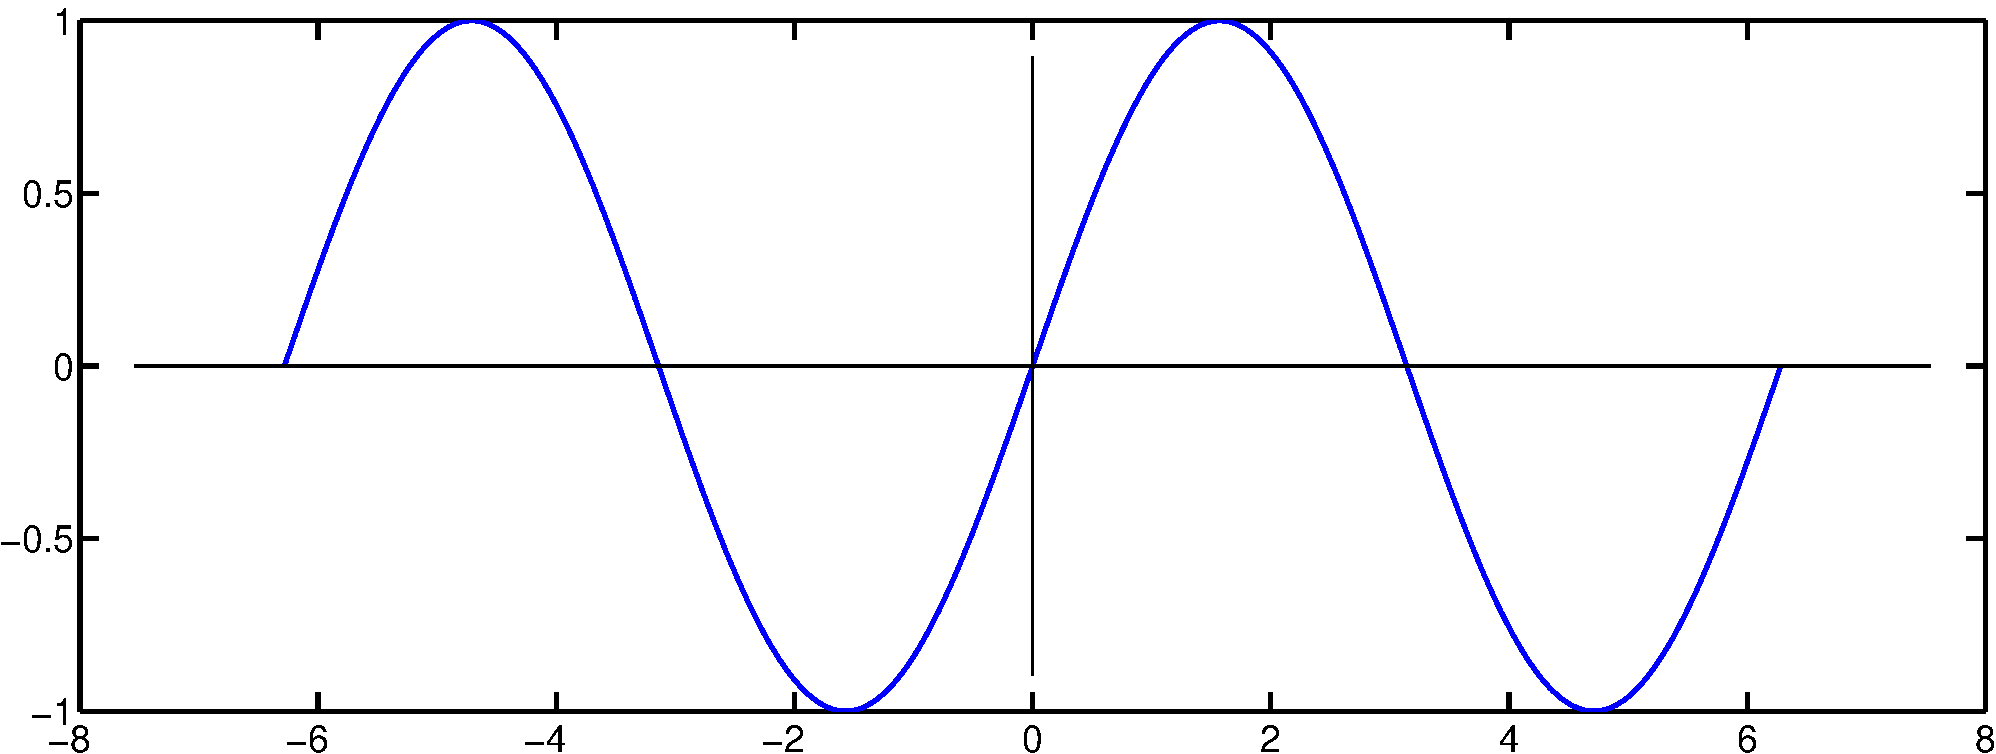
\includegraphics[width=9cm]{Matlab/sin}
\end{center}

This function is \Emph{not} invertible, because it is not one-to-one.
However, if we restrict the domain to $[-\frac{\pi}{2},
\frac{\pi}{2}]$, then it is invertible.

}

\rblock
\frame{
\begin{columns}[c]
\column{0.5\textwidth}
\begin{block}{Inverse $\sin$ function}
The inverse of the \eq{\sin} function on $[-\pi/2, \pi/2]$ is
denoted \eq{\sin^{-1}(x)} or \eq{\arcsin(x)}
\[ y = \sin(x) \Longleftrightarrow x = \sin^{-1}(y).\]
\end{block}

\vspace{1cm}

\pause 
The notation $\arcsin$ is still often used text books, but we'll use
\eq{\sin^{-1}}.  Take care not to confuse this with $1/\sin(x)$.

\column{0.5\textwidth}

\begin{center}
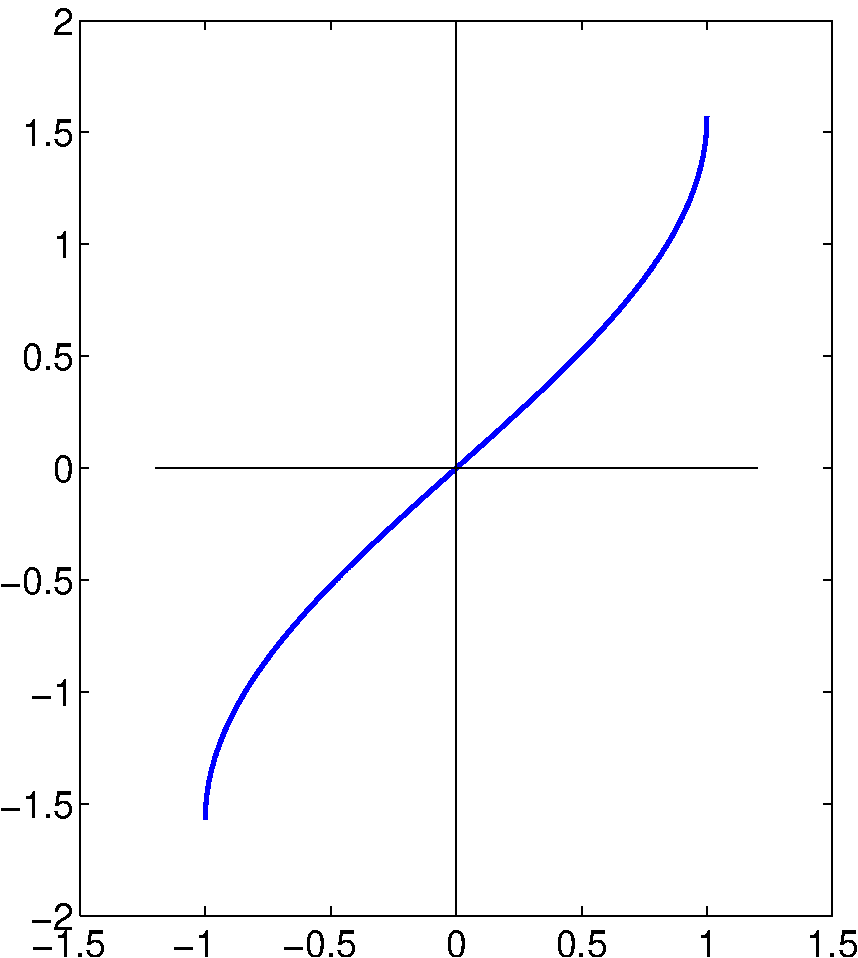
\includegraphics[width=5cm]{Matlab/asin}
\end{center}


\end{columns}
}

\frame{
\begin{example}
Simplify \eqd{\tan\big( \sin^{-1}(x)\big)}.
\end{example}


\vspace{3cm}
}

\subsection{$\sin^{-1}, \cos^{-1}$ and $\tan^{-1}$}

\frame{

We can also define the inverse of the \eq{\cos} and \eq{\tan}
functions. 

The derivatives of the inverse trig functions are

\begin{center}
\begin{tabular}{c|c}
$\boldmath{\alert{ f(x)}}$ & $\displaystyle \boldmath \alert{\frac{d}{dx} f(x) } $\\ \hline
$\sin^{-1}(x)$ &\\ \hline
$\cos^{-1}(x)$ &\\ \hline
$\tan^{-1}(x)$ & 
\end{tabular}
\end{center}


\pause
(See p41 in the Mathematical Tables).

}

\section{Euler Formula}

\frame{
For complex numbers, it is possible to express \eq{e^x} in terms of
\eq{\sin} and \eq{\cos}:
\[
e^{i x} = \cos(x) + i \sin(x), \quad \text{ where } i =\sqrt{-1}.
\]
This is known as \Emph{Euler's Formula}.

Using that \eq{\cos} is an \Bf{even} function, and \eq{\sin} is an \Bf{odd}
function, we get:

\vspace{3cm}

}

\frame{
\begin{example}
Use that
\[
\cos(x) = \frac{1}{2}\big(e^{ix} + e^{-ix}\big)
\]
to find \eq{\frac{d}{dx}\cos(x)}.
\end{example}
\Bf{Solution:}
\vspace{3cm}

}


\frame{
\begin{exercise}
Use that
\[
\sin(x) = \frac{-i}{2}\big(e^{ix} - e^{-ix}\big)
\]
to find \eq{\frac{d}{dx}\sin(x)}.
\end{exercise}


}

\end{document}
\bblock
\section{The Hyperbolic Functions}

\frame{

\begin{definition}[Hyperbolic Functions]
  The \Bf{Hyperbolic cosine and sine functions} are defined as
\[
\cosh(x) = \frac{1}{2}{e^x - e^{-x}}, 
\qquad 
\text{ and } 
\sinh(x) = \frac{1}{2}{e^x - e^{-x}}, 
\]
\end{definition}
\begin{center}
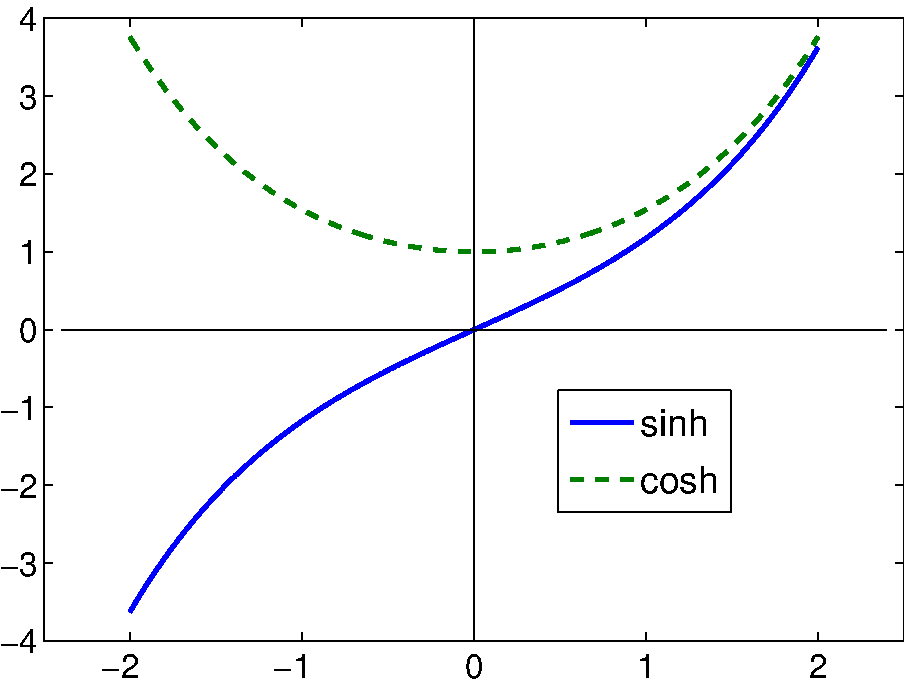
\includegraphics[width=6cm]{Matlab/sinh}
\end{center}

}

\frame{

\begin{block}{}
The \eq{\tanh} and \eq{cotanh} functions can be defined 
\[ \tanh x = \frac{\sinh x}{\cosh x} \]
\[ \coth x = \frac{1}{\tanh x} = \frac{\cosh x}{ \sinh x}. \]
\end{block}
\begin{center}
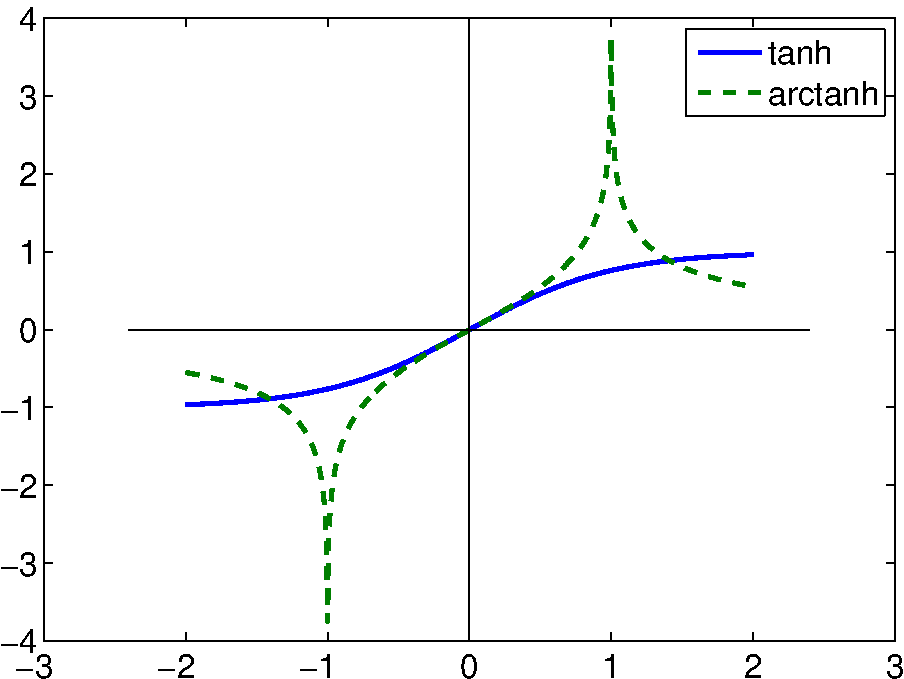
\includegraphics[width=5.6cm]{Matlab/tanh}
\end{center}




}
\rblock
\frame{

\begin{exercise}

Recall that
\[
\cos^2 x + \sin^2 x = 1.
\]

Show that
\[
\cosh^2 x - \sinh^2 x =1.
\]

\end{exercise}
}


\frame{
The previous slide highlights a difference between the hyperbolic and
trigonometric functions. Nonetheless, they have much in common:


\begin{itemize}[<+->]
\item $\cosh (x+y) = \cosh x \cosh y + \sinh x \sinh y$
\item $\sinh (x+y) = \sinh x \cosh y + \cosh x \sinh y$
\end{itemize}

\Bf{Example:}

\vspace{2cm}

}

\frame{

\begin{theorem}
\begin{itemize}
\item $\frac{d}{dx}(\sinh x) = \cosh x$
\item $\frac{d}{dx} (\cosh x) = \sinh x$
\end{itemize}
\end{theorem}

\Bf{Proof:}

}

\frame{
\begin{example}
 Differentiate $\tanh x$.
\end{example}
\Bf{Solution:}


\vspace{2cm}

}
\end{document}




\end{document}


\subsection{The derivative of the inverse}

\frame{
Suppose we have a function $f$ and its inverse $f^{-1}$. Can we
express \eqd{\frac{d}{dx}f^{-1}(x)} in terms of $f'$ and $f^{-1}$?\\
The trick is to use \Emph{implicit differentiation} (Stewart, \S3.5) 

\vspace{3cm}

\pause

So we see that 
\begin{block}{}
\[ \frac{d}{dx}f^{-1}(x) = \frac{1}{f'\big(f^{-1}(x)\big)}. \]
\end{block}
}


\end{document}
\subsection{$\frac{d}{dx}\exp(x)$}

\frame{
Perhaps the most important property of the exponential function can be
deduced as follows:

\vspace{4cm}

\pause
\begin{alertblock}{}

\[ \frac{d}{dx}\exp(x) = \exp(x).\]
So the exponential function is its own derivative!
\end{alertblock}

}


\end{document}

